\begin{problema}
\mbox{}
    \begin{enumerate}
        \item[(i)]
            Ejecute y explique la funci\'on del siguiente c\'odigo en Octave. Comente qu\'e 
            teoremas del curso (y del curso de probabilidad) son importantes para interpretar 
            la figura.
            \tiny
            \texttt
            {
                \lstinputlisting[caption=]{tarea3/problema3_4/polya2.R}
            }
            \normalsize
            (Conmigo se negó a brincar de linea. Tuve que hacerlo diminuto para que apareciera el código completo.)\par\null
        
        \item[(ii)]
            Ejecute y explique la funci\'on del siguiente c\'odigo en Octave. 
            Incluya una gr\'afica en la que la longitud de la variable k sea mayor a 1000. 
            (Puede modificar el programa...) En la gr\'afica observara un esbozo de la 
            trayectoria de un proceso de ramificaci\'on continuo (en una escala distinta...).
            \texttt{
                \lstinputlisting[caption=]{tarea3/problema3_4/binaryGW.R}
            }
    \end{enumerate}
\end{problema}

\begin{proof}
    \subsection{Inciso (i)} \label{problema3_4:inciso1}
    \emph
{
            Ejecute y explique la funci\'on del siguiente c\'odigo en Octave. Comente qu\'e 
            teoremas del curso (y del curso de probabilidad) son importantes para interpretar 
            la figura.
            \tiny
            \texttt
            {
                \lstinputlisting[caption=]{tarea3/problema3_4/polya2.R}
            }
            \normalsize
}

\afterstatement\pn

En el código se simulan \texttt{10000} procesos de urnas de Póyla con \texttt{1000} iteraciones cada uno.\pn

\texttt{n} es el número de juegos por proceso.\pn

\texttt{m} es el número de simulaciones.\pn

\texttt{u} es una matriz de probabilidades. En este caso, la 
entrada \texttt{(i,j)}, es el ``resultado'' del turno
\texttt{j} en el proceso \texttt{i}.\pn

\texttt{r} y \texttt{v} son el número de pelotas rojas y verdes 
(respectivamente) con las que comienza cada proceso. Esto se deduce 
de la manera en que se obtienen las proporciones iniciales \texttt{r/(r+v)}.\pn

\texttt{c} es la constante de bolas que se agregan en cada paso del proceso. Esto se deduce en la manera que se obtiene la
\texttt{i}-ésima proporción (se divide entre \texttt{r+v+i*c} es decir, el número de pelotas en el \texttt{i}-ésimo paso es
el número de bolas iniciales más \texttt{i} veces \texttt{c}).\pn

\texttt{x} es una matriz en cuyas columnas se representan la sucesión de proporciones de 
bolas rojas en cada proceso. La instrucción \texttt{ones(1,m)} genera una matriz de 
\texttt{1$\times$m} con unos en todas las entradas. Al multiplicar por \texttt{r/(r+v)} 
se obtiene una matriz con el valor \texttt{r/(r+v)} en todas sus entradas. En otras palabras, 
\texttt{x} es el vector de proporciones de bolas rojas iniciales para cada proceso.\pn

El ciclo \texttt{for} es para calcular las sucesiones de proporciones. Se puede comparar 
con el del problema [\ref{problema2_2}] o
su versión corregida que se encuentra en la solución de dicho problema.\pn

\texttt{y} es la colección de proporciones de bolas rojas finales de cada proceso. Para 
fines de graficación, se ordenan con el
comando \texttt{sort}.\pn

En la penúltima linea se ve el comando \texttt{plot} a quien se le pasan la colección 
de proporciones finales y una representación de una función beta con parámetros de forma 
(shape parameters) \texttt{r/c} y \texttt{v/c}.\pn

La siguiente gráfica es el resultado de una ejecución del algoritmo anterior. En azul, se 
muestra el resultado experimental de las \texttt{10000} iteraciones del proceso. En verde 
la gráfica de una distribución Beta con parámetros de forma \texttt{r/c} y \texttt{v/c}.\pn

\begin{center}
    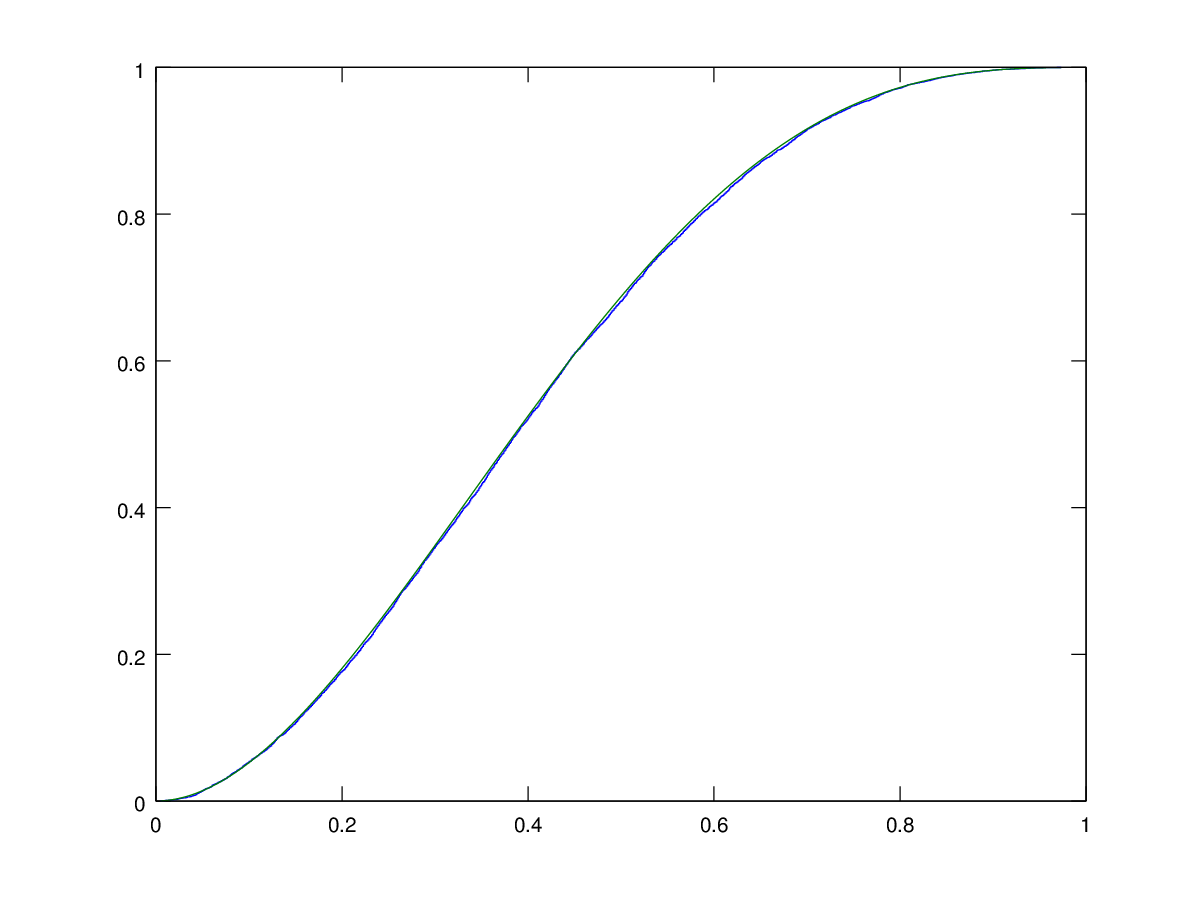
\includegraphics[width=8cm]{tarea3/problema3_4/poylaBeta.PNG}\pn
    Gr\'afica del histagrama de los radios ``finales'' de \texttt{10000} iteraciones del proceso 
	de urnas de P\'oyla (azul). En contraste con una distribución Beta (verde).\pn
\end{center}

En clase se demostró que los radios esperados tenían distribución Beta con los parámetros 
ya mencionados. En la gráfica se puede apreciar el parecido del resultado experimental con el teórico.\pn

P.S. \texttt{tic}, \texttt{toc} son funciones de octave para medir el tiempo de ejecución. En este caso
la ejecución duró cerca de un minuto. Lo cual era de esperarse, se realizaron poco más de \texttt{120,000,000} operaciones
y además, construir un gráfico con una retícula de \texttt{10000} puntos también es un proceso computacionalmente caro.
    \newpage

    \subsection{Inciso (ii)} \label{problema3_4:inciso2}
    \emph{
    Ejecute y explique la funci\'on del siguiente c\'odigo en Octave. 
    Incluya una gr\'afica en la que la longitud de la variable k sea mayor a 1000. 
    (Puede modificar el programa...) En la gr\'afica observara un esbozo de la 
    trayectoria de un proceso de ramificaci\'on continuo (en una escala distinta...).
    \texttt{
        \lstinputlisting[caption=]{tarea3/problema3_4/binaryGW.R}
    }
}

\afterstatement\pn

El código simula un proceso de Galton-Watson.\pn

\texttt{k = [10]} significa que al inicio habrá 10 individuos.\pn

\texttt{aux} es la última población obtenida. \texttt{binornd(aux, .5)} es una instrucción de Octave en la que
de un conjunto de \texttt{aux} elementos, escoge a cada uno con probabilidad \texttt{.5}. El resultado
es el número de elementos seleccionados. Multiplicar esto por \texttt{2} se puede interpretar como que
antes de morir, cada individuo seleccionado tiene dos hijos.\pn

\texttt{k = [k; 2*binornd(aux, .5)]} está agregando al vector \texttt{k} una nueva entrada. La entrada,
es la nueva población, resultante de que cada individuo seleccionado tiene dos hijos antes de morir y cada
elemento no seleccionado muere sin tener decendientes.\pn
 
A continuación, una gráfica con una ejecución de este algoritmo comenzando con \texttt{10} individuos
y terminando con \texttt{0} individuos después de un poco más de \texttt{12000} iteraciones.

\begin{center}
    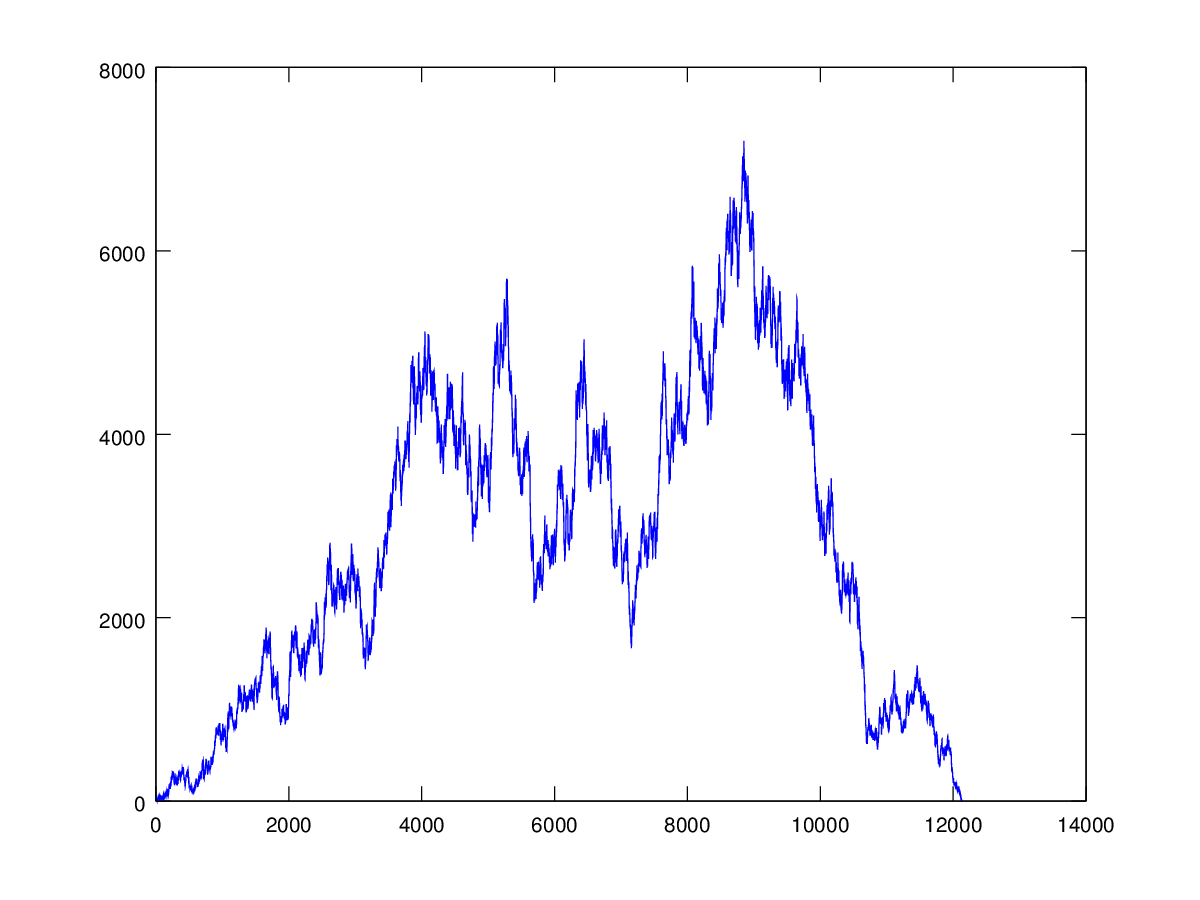
\includegraphics[width=8cm]{tarea3/problema3_4/galtonWatson.PNG}
    
    Gr\'afica de una ejecuci\'on del proceso de extinci\'on de Galton-Watson 
    Par\'ametros:\par
    10 individuos\par 
    La probabilidad de que un individuo tenga $2$ hijos es $\frac{1}{2}$\par
    La probabilidad de que un individuo tenga $0$ hijos es $\frac{1}{2}$.\pn
\end{center}

La esperanza de número de decendientes que tiene un individuo, es \texttt{1}. Es decir,
este proceso de Galton-Watson es crítico. En clase se demostró que los procesos Galton-Watson
críticos se extinguen con probabilidad \texttt{1}. La gráfica arriba mostrada es de una corrida
del algoritmo que más iteraciones duró antes de extinguirse, el algoritmo, se corrió
\texttt{200,000} veces y, en todos los casos se extingió la población. Esto es consistente con
con el resultado teórico (en todos los casos, de un conjunto de \texttt{200,000}, la población se extinguió).\pn

A continuación, una gráfica resultante del mismo algoritmo, pero con una población inicial de \texttt{1000} individuos.
que se extingue después de \texttt{20,000} iteraciones. Cabe mencionar que esta corrida fue más ``suertuda'' que la
representada en la gráfica anterior. Muchas de las corridas del algoritmo sin modificar superaron una población de
\texttt{1000} individuos en algún momento y después de eso, nunca duraron tanto como este otro.

\begin{center}
    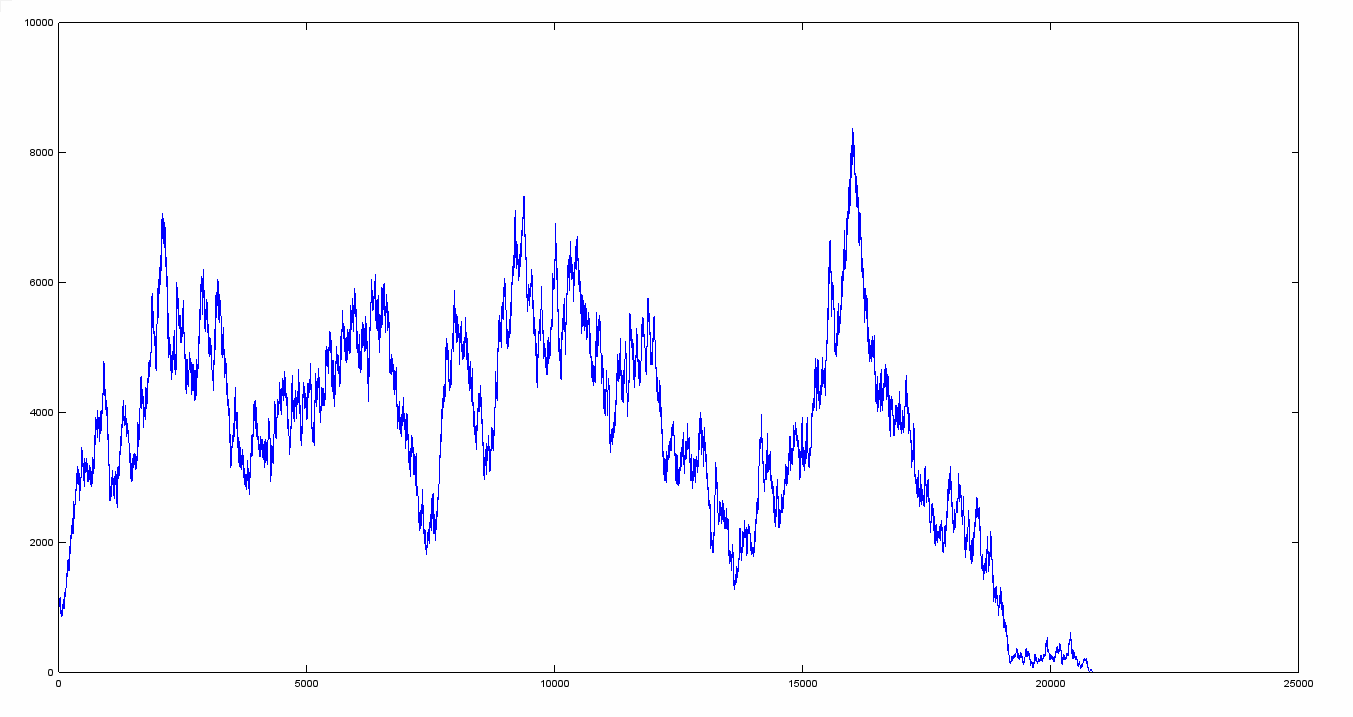
\includegraphics[width=12cm]{tarea3/problema3_4/galtonWatsonEmpezandoEn1000.PNG}
    
    Gr\'afica de una ejecuci\'on del proceso de extinci\'on de Galton-Watson 
    Par\'ametros:\par 
    1000 individuos iniciales \par
    La probabilidad de que un individuo tenga $2$ hijos es $\frac{1}{2}$ \par
    La probabilidad de que un individuo tenga $0$ hijos es $\frac{1}{2}$.\pn
\end{center}

P.S. El algoritmo modificado se incluye bajo el nombre de \par
\texttt{BinaryGWModificado.R}. (Incluí un candado para que el algoritmo terminara si 
superaba un millón de iteraciones, nunca se alcanzó dicho límite).
\end{proof}